\documentclass[]{report}
\usepackage[margin=1in]{geometry}
\usepackage{graphicx,wrapfig}


% Title Page
\begin{titlepage}
\centering
\title{Identifying Hand Hygiene Using Deep Neural Networks}
\author{James H. Edwards \\ 
	advised by Dr. Valerie Galluzzi, Dr. Matthew Boutell, and Dr. Klaus Baer\\
	\\
	\\
	A thesis submitted in partial fulfillment of the requirements for the \\
	Bachelor of Science degrees in International Computer Science \\
	at the Rose-Hulman Institute of Technology and Hochschule Ulm.}
	
\end{titlepage}
\begin{document}
\maketitle
\tableofcontents

\begin{abstract}
	Both machine and deep learning are growing fields of computer science that are rapidly increasing in relevance to our society. One compelling field of application is in the healthcare industry, and specfically in hospitals. Systems can be designed to help and improve the lives of patients with particular diseases or disabilities, and systems can even be trained to diagnose complicated symptoms or to otherwise aid doctors in their duties. The experiment used in this project was originally conducted by Dr. Valerie Galluzzi, who used custom 3-D wrist accelerometer sensors in order to measure healthcare worker compliance to hand-washing guidelines. The contribution of this work was to take the data and use deep neural networks to generate models that can predict when a novel sample is performing hand hygiene. After trying out various neural network configurations, the best model attained over 83\% accuracy with over 81\% recall.
\end{abstract}

\chapter{Background}

This part of the thesis provides an introduction to the concepts of deep learning and neural networks, followed by a summary of other recent work in this field. It will help the reader become familiar with the works I consulted in order to better understand my topic and explain the reasoning behind deep learning in case that is necessary for the reader.


\section{Hand Hygiene}

One of the most effective techniques to prevent the spread of infection in hospitals is having healthcare workers (such as doctors and nurses) follow proper hand hygiene guidelines \cite{Galluzzi}. To help achieve this task, many organizations, including the World Health Organization (WHO), have created standards and guides for how to properly perform hand hygiene. They have set out the ``5 Moments of Hand Hygiene'' \cite{WHO}:
\begin{enumerate}
	\item Before touching a patient
	\item Before clean/aseptic procedure
	\item After body fluid exposure risk
	\item After touching a patient
	\item After touching patient surroundings
\end{enumerate}

\begin{figure}
	\centering
	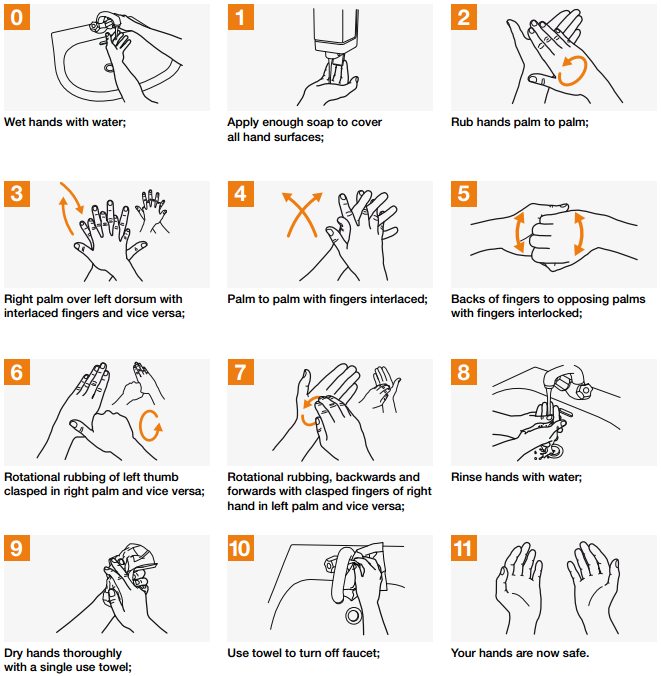
\includegraphics[width=0.5\textwidth]{../images/handhygiene-summary}
	\caption{Hand Hygiene Technique with Soap and Water \cite{who2}}
	\label{hh-guidelines}
\end{figure}

Because proper hand hygiene is so important, it is worthwhile to develop a system to ensure that healthcare workers are complying with these guidelines and following proper techniques. Therefore Dr. Galluzzi developed a system of wrist-attached sensors to measure the three axes of acceleration of a user's hands. For her Ph.D. dissertation she analyzed the data gathered from several healthcare workers during their shift, collecting data both from ``hand hygiene'' activities (i.e. actually washing one's hands) and ``not hand hygiene'' activities (e.g. unwrapping a piece of candy, tying one's shoes, or simply walking around) \cite{Galluzzi}. She then used machine learning techniques to try to identify particular hand hygiene motions such as the ``fingertip scrub'' and other actions outlined by the WHO \cite{Galluzzi}. One example of the guidelines are shown in Figure~\ref{hh-guidelines}.




\section{Related Work}

This section gives a brief overview of the current uses of machine and deep learning in the healthcare field.


\section{Deep Learning}

In the Nature article titled ``Deep Learning,'' three pioneers of deep learning and neural networks, Yann LeCun, Yoshua Bengio, and Geoffrey Hinton write about the big picture and history of deep learning. They state that the key differentiation between machine learning and deep learning is ``these layers of features [in deep learning] are not designed by human engineers: they are learned from data using a general-purpose learning procedure'' \cite{ThreeGiants}. 

In general, deep learning uses layers of interconnected ``neurons'' in order to try to simulate the brain, as shown in Figure~\ref{neural-model}. In this example, each $x_{i}$ represents an input value and each $w_{i}$ represents a weight. These weights are initially random but are adjusted through a process known as backpropagation (i.e. the ``learning'' in ``deep learning''). The $w_{i}*x_{i}$ values are summed together and added to $b$, which is the bias value, and adds a linear offset to the model. Each input $x_{i}$ has a corresponding output, called $y_{i}$. These values are then used in a loss function to minimize the cross-entropy between the estimated output value and the real output value, which for the example of one single input multiplied by one weight value is: $$-\sum_{i} (w_{i}*x_{i})*\ln(y_{i}) $$
\begin{figure}
	\centering
	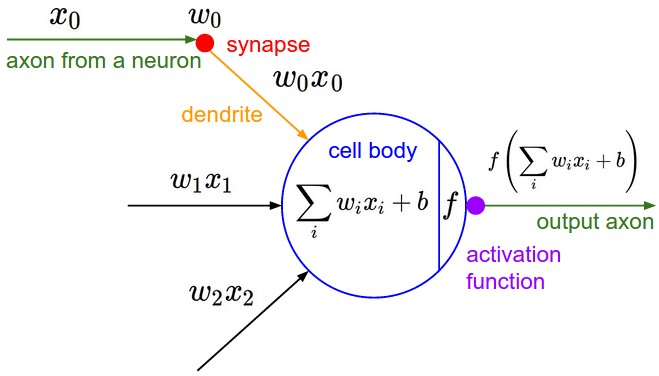
\includegraphics[width=0.5\textwidth]{../images/neuron_model}
	\caption{Each component of the neural network model simulates an element of the brain \cite{karpathy}}
	\label{neural-model}
\end{figure}

Backpropagation uses the gradient of this loss function to adjust the weights. This process is repeated, usually for a certain number of steps, with the result being that the multiplications and summations hopefully emulate the actual values corresponding to the input values. In practice these models have thousands to millions of $(x_{i}, y_{i})$ pairs and usually have a few hundred nodes in each of multiple layers, and the data is put into vectors or matrices to simplify the code. 

%The authors also go into detail about the finer points of stochastic gradient descent (SGD) and talk about how using small sets of examples is better than going one example at a time (essentially because things averaging out is better). 
In order to both improve results and speed, it is now common to use stochastic gradient descent (SGD) during training instead of performing a gradient descent for every training example. Because larger sets of data perform better (simply due to the existence of more examples, which can perhaps be more generalized), SGD improves training time by following the gradient descent of a ``minibatch'' of examples at a time, instead of a single example \cite{Goodfellow-et-al-2016,ThreeGiants}. While this method loses a bit of particularity, it therefore gains in generalization over the many training examples which are utilized.


When multiple layers are connected to each other in a deep network, these functions may tend to collapse together because the total function is simply a series of affine transformations. Thus it is important to use a nonlinear output function as the input to the next layer. Common choices are the hyperbolic tangent function or the logistic sigmoid activation function. A more recent development is the Rectified Linear Unit (ReLU) function, shown in Figure~\ref{relu}. The ReLU function is clearly nonlinear but also has a simple and easy gradient to calculate, so it is now the standard function used \cite{Goodfellow-et-al-2016,ThreeGiants}.

\begin{figure}
	\centering
	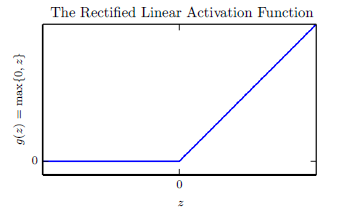
\includegraphics[width=0.4\textwidth]{../images/relu}
	\caption{The ReLU function \cite{Goodfellow-et-al-2016}}
	\label{relu}
\end{figure}



Another type of neural network has the name of Convolutional Neural Networks (CNNs). These networks are normally used for image data, and use different types of layers, namely convolutional layers, pooling layers, and fully-connected layers. Convolutional layers use patches of weights, usually much smaller than an image but also ``deeper'' in the third dimension, which then help identify different parts of an image, shown in Figure~\ref{convolution-exp}. CNNs have been hugely successful in the field of image recognition, which also aids in the effectiveness of self-driving cars. CNNs are now even able to caption images, showing that the networks really ``understand'' patterns in the picture and do not just see pixels of various colors.


\begin{figure}
	\centering
	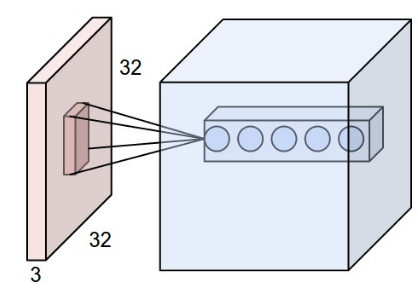
\includegraphics[width=0.4\textwidth]{../images/convolutions2}
	\caption{A convolutional layer takes an adjacent set of values and extends the depth dimension \cite{karpathy}}
	\label{convolution-exp}
\end{figure}


The website ``Neural Networks and Deep Learning,'' written by Michael Nielsen, provides a excellent and quite detailed introduction to deep learning by explaining the Mixed National Instrument of Standards and Technology (MNIST) dataset and networks that have high accuracy in classifying the dataset \cite{NNDL}. Nielsen mentions that perceptrons (another name for a node in a neural network) multiply their inputs by a particular weight and then a bias is added, and then that value is output (perhaps into the sigmoid or ReLU function). Technically a cost function, usually Mean Squared Error (MSE) or Cross Entropy (CE), is used to find the error between the projected outputs and the real outputs, and then the weights and biases are adjusted through backpropagation. He also goes into great detail about backpropagation and explains how putting everything into vectors and then using a graph of calculations can make the calculations simpler and make it possible to compute all of the partial derivatives in one pass. He explains some types of regularization, namely L2 (attempting to limit the total value of the weight matrix), dropout (randomly removing nodes in a network), and early stopping, all of which are designed to avoid overfitting / overtraining.


\subsection{Video-Based Systems}

While my project used acceleration data, I found it helpful to look into the research utilizing video data in order to learn about another set of deep learning applications to healthcare.

Neverova, Wolf, Taylor, and Nebout claim that gesture identification has several challenges: ``cultural and individual differences in tempos and styles of articulation, variable observation conditions, ..., [and] infinitely many kinds of out-of-vocabulary motion,'' among others \cite{Neverova}. Their model, a convolutional neural network which took in intensity and depth video, along with ``articulated pose information extracted from depth maps'' won the 2014 ChaLearn Challenge for Multi-modal Gesture Recognition \cite{Neverova}. The general system used a skeletal mapping program to try to identify the various parts of the body from a video/image based on different frame stride lengths. Their main design improvement was to use a custom ``ModDrop'' (Modular Dropping) process, which made the system more effective by separating or combining the different types of inputs at particular points in the pipeline \cite{Neverova}. 

Starner, Weaver, and Pentland worked on a system to recognize American Sign Language in real time. They designed two systems which used Hidden Markov Models and ``tracked unadorned hands'' to classify signs based on a 40 word lexicon \cite{Starner98}. One system was a camera on a desk looking at a signer, and the other was a camera on a hat worn by a signer (trying to identify his own signs). By using a ``strong part-of-speech grammar'' they achieved a test accuracy of over 87\% for the first system and over 97\% for the second \cite{Starner98}. The authors did express some concern over the potential issues with increasing the possible word-count as well as the variance between different signers and mentioned that perhaps gloves or finger sensors may be needed, as well as gathering much more data overall \cite{Starner98}.

Shin and Sung claim that gesture recognition is of vital importance for wearables. These researchers developed ``dynamic hand gesture recognition techniques,'' one of which used a CNN and an RNN combined taking in video data, while the other only used an RNN but used accelerometer data \cite{ShinS16}. The RNN that used accelerometer data uses LSTMs with the standard 3 gates (input, forget, output). However, trying to compress the floating points came at significant accuracy cost. With only two bits of quantization, the error rate was 32.77\%. Three bits gave an error rate of 28.69\% but 4 bits gave 11.43\%. Doing so reduced the memory requirements by over 90\% \cite{ShinS16}. 

\subsection{Sensor-Based Systems}

Bulling, Blank, and Schiele set out to make a comprehensive overview of the Human Activity Recognition (HAR) problem with ``body-worn inertial sensors'' \cite{Bulling}. They first mention several fields that would benefit from activity recognition: the industrial, sports, entertainment, and healthcare sectors \cite{Bulling}. They noted several applications and devices such as the Wii and Kinects as well as the Nike+ shoes which help track activity. They mentioned several key challenges that the field of HAR has: no clear definition of specific activities, the various possible composition of sensors, and the specific evaluation metrics for each application. Other challenges include intraclass variability, interclass similarity, the Null class problem, the diversity of physical activities, class imbalance, the annotation of ground truth, data collection and experiment design, variability in sensors, and system design. I can certainly understand how these issues can cause major problems in identification. For my data I am not exactly sure how much effect intraclass variability has in my classification system, however people certainly wash their hands in different ways, perhaps by doing motions in different orders. Being left- or right-handed also could play a role. Of huge importance to my work is dealing with class imbalance, because the dataset is over 95\% ``Not Hand Hygiene'' samples. The authors also propose a system model called the Activity Recognition Chain which has the following steps: data acquisition, signal preprocessing, segmentation, feature extraction and selection, training, and classification \cite{Bulling}. 

Hammerla, Halloran, and Plötz provide another overview of how deep learning techniques are applied to HAR. They state that the main technique of HAR ``includes sliding window segmentation of time-series data captured with body-worn sensors, manually designed feature extraction procedures, and a wide variety of (supervised) classification methods'' \cite{Hammerla}. Their paper applies various types of neural networks to covering 3 problems: ``manipulative gestures, repetitive physical activities, and a medical application ... in Parkinson's disease'' \cite{Hammerla}. One of the networks had five hidden layers and used either dropout or max-in norm for regularization with mini-batches of size 64. This network achieved just over 90\% accuracy on the repetitive gesture dataset but got almost 60\% on the other two datasets; the other networks did better on average over the three problems \cite{Hammerla}.

Lester, Choudhury, and Borriello designed a ``personal activity recognition system'' to be used by anyone \cite{Lester2006}. They used a single sensor that could be put in different locations on the body but then had multiple types of sensors. Twelve subjects performed 8 activities over a few days ``carrying a collection of sensors worn in three different locations on the body.'' The researchers wanted to find out if the location of the sensor mattered, how much values changed between users, and how many sensors are actually required to ``recognize a significant set of basic activities'' \cite{Lester2006}.
Using Hidden Markov Models they achieved between 80\% and 90\% accuracy for each sensor location, as well as all sensors combined \cite{Bulling}. They found that the location of the sensor did not really matter, the system worked well on a new subject, and only 3 types of sensors were needed to do the job well: audio, barometric pressure, and accelerometer.


\chapter{Experiments}

Now that the reader has an introduction to the neural networks and a view on the current research in deep learning in the healthcare field, I will describe the experiment I undertook. It begins with a discussion of the data and some issues I encountered, the models I developed to train, and other deep learning techniques I used to increase the accuracy of my models.

\section{Initial Steps}

My project is a continuation of the work of Dr. Valerie Galluzzi, who did her dissertation on using machine learning techniques to identify if various healthcare workers were being compliant with the guidelines of the World Health Organization. She and her team worked to develop custom wrist-wearable acceleration sensors, which sent data to a separate device. The data could be offloaded for investigation. I was given most of the data she used, which consisted of many samples from 116 healthcare workers in a hospital \cite{Galluzzi}. These acceleration values were sampled at 100 Hz, and measured the X, Y, and Z acceleration values for each hand for varying lengths of time (the data for each hand was recorded on separate devices but the values were stored together). 

\begin{figure}
	\centering
	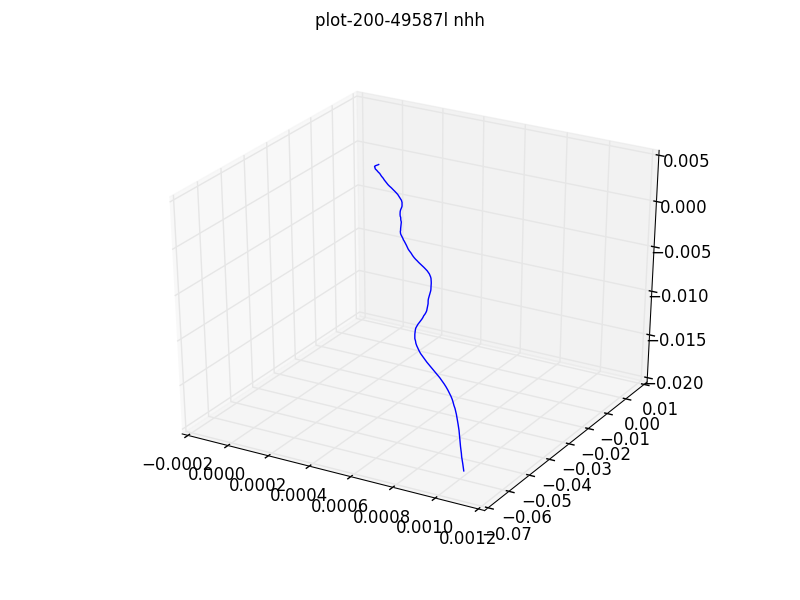
\includegraphics[width=0.5\textwidth]{../code/plots/plot-200-49587l}
	\caption{Plot of a Not Hand Hygiene Sample}
	\label{nhh-plot}
\end{figure}

\begin{figure}
	\centering
	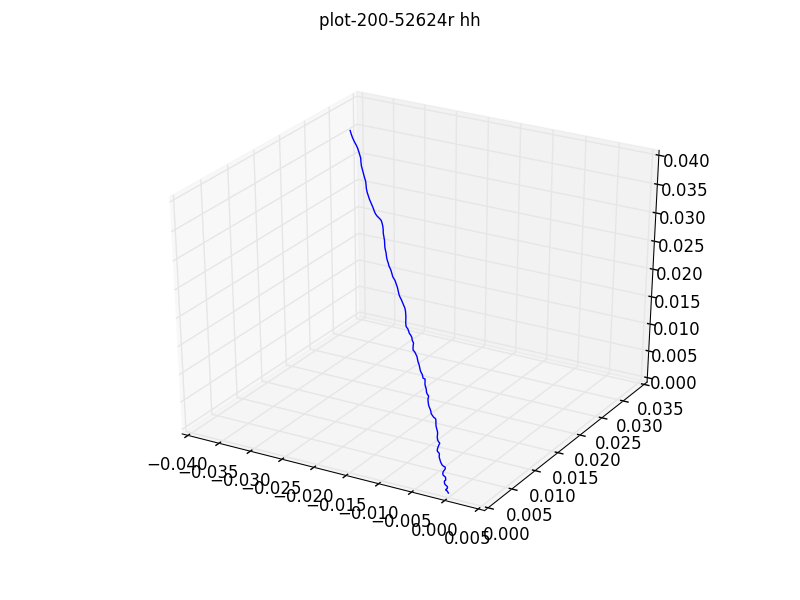
\includegraphics[width=0.5\textwidth]{../code/plots/plot-200-52624r}
	\caption{Plot of a Hand Hygiene Sample}
	\label{hh-plot}
\end{figure}

Figure~\ref{nhh-plot} and Figure~\ref{hh-plot} show plots of a Not Hand Hygiene sample and a Hand Hygiene sample respectively. These two images were constructed by integrating the acceleration values and assuming an initial position and velocity of zero. The small differences between the paths of the hands in these plots can illustrate that it is not always straightforward to identify a Hand Hygiene sample from a Not Hand Hygiene sample.

\begin{figure}
	\centering
	\begin{tabular}{| l | l |}
		\hline
		Participant: & Random ID \\ 
		\hline
		Handedness: & h \\ 
		\hline
		Job: & o \\ 
		\hline
		Rate: & 100 \\ 
		\hline
		Samples: & \begin{tabular}{l | l}
			Left: & \begin{tabular}{l | l}
				0: & \begin{tabular}{l | c}
					Sample & \textless String of ``X,Y,Z'' values \textgreater\\
					\hline
					Class & ``HH'' or ``NHH''\\
					%\hline
				\end{tabular}\\ \hline
				1: & \begin{tabular}{l | l}
					Sample & \textless String of ``X,Y,Z'' values \textgreater\\
					\hline
					Class & ``HH'' or ``NHH''\\
					%\hline
				\end{tabular}\\ \hline
				\vdots & \vdots\\
			\end{tabular}\\
			\hline
			Right: & \begin{tabular}{l | l}
				0: & \begin{tabular}{l | c}
					Sample & \textless String of ``X,Y,Z'' values \textgreater\\
					\hline
					Class & ``HH'' or ``NHH''\\
					%\hline
				\end{tabular}\\ \hline
				1: & \begin{tabular}{l | l}
					Sample & \textless String of ``X,Y,Z'' values \textgreater\\
					\hline
					Class & ``HH'' or ``NHH''\\
					%\hline
				\end{tabular}\\ \hline
				\vdots & \vdots\\
			\end{tabular}\\
		\end{tabular}
	\end{tabular}
	\caption{A Visual Explanation of the Original JSON Data}
	\label{jsonformat}
\end{figure}


I initially worked on reorganizing the data. It had been given to me in a JSON file shown in Figure~\ref{jsonformat}, whereas it is much easier to work with CSV files that can be imported in Pandas, a Python module that can be combined with TensorFlow (Google's Deep Learning API). The reader will please note that the sample labels are abbreviated from ``Hand Hygiene'' and ``Not Hand Hygiene'' to ``HH'' and ``NHH'' respectively; these abbreviations will be used throughout the rest of this paper. Once I had a Python script which converted the data to CSVs, I then made a second Python script to load the data from the CSV files and put the various acceleration data points into separate X, Y, and Z matrices. These matrices served as the inputs to the Tensorflow models.

\begin{figure}
	\centering
	\begin{tabular}{ ccc }
		%\hline
		$X$ & $Y$ & $Z$\\
		%\hline
		$$ 
		\left[ \begin{array}{cccc}
		x_{1} & x_{2} & ... & x_{n} \\
		x_{n+1} & x_{n+2} & ... & x_{2*n} \\
		\vdots & & \ddots & \\
		\end{array} \right] 
		$$
		&
		$$ 
		\left[ \begin{array}{cccc}
		y_{1} & y_{2} & ... & y_{n} \\
		y_{n+1} & y_{n+2} & ... & y_{2*n} \\
		\vdots & & \ddots & \\
		\end{array} \right] 
		$$
		&
		$$ 
		\left[ \begin{array}{cccc}
		z_{1} & z_{2} & ... & z_{n} \\
		z_{n+1} & z_{n+2} & ... & z_{2*n} \\
		\vdots & & \ddots & \\
		\end{array} \right] 
		$$\\
%		$x_{0}, x_{1}, ... x_{N-1}$ & $y_{0}, y_{1}, ... y_{N-1}$ & $z_{0}, z_{1}, ... z_{N-1}$ \\
%		\hline
%		$x_{N}, x_{N+1}, ... x_{2N-1}$ & $y_{N}, y_{N+1}, ... y_{2N-1}$ & $z_{N+1}, z_{N+2}, ... z_{2N-1}$ \\
%		\vdots & \vdots & \vdots \\
		%\hline
	\end{tabular} 
	\caption{A Visual Explanation of the Data Processed into Matrices with Width N}
	\label{matrixformat}
\end{figure}
The layout of the preprocessed data I used for the majority of the project is shown in Figure~\ref{matrixformat}. I split each dimension into its own matrix. I used each of $n= \lbrace5,25,50,75,100,125,150,175,200,225,250\rbrace $ during testing of the models, in order to see how using different window lengths affected the outcome.

Because of the way the data was collected, I did not actually have a continuous stream of data; that is, each sample did not exactly or directly take place immediately before or after another sample. Therefore I had to work with the individual slices provided to me, rather than a constant stream of values I could divide up any way I wished. This split of the data meant that I unfortunately could not truly look at slicing an entire session's data into different samples, but did also allow for simple labelling of the samples as either ``HH'' (Hand Hygiene) or ``NHH'' (Not Hand Hygiene).

\begin{table}
	\centering
	\label{supersamples}
	\begin{tabular}{|c|r|r|r|r|r|r|r|r|r|r|r|}
		\hline
		Sample Length          & 5 & 25 & 50 & 75 & 100 & 125 & 150 & 175 & 200 & 225 & 250 \\
		\hline
		Supersample Coefficient & 1 & 5  & 8  & 10 & 13 & 16  & 18  & 23  & 25  & 27  & 29 \\
		\hline
	\end{tabular}
	\caption{Table of Supersample Values}
\end{table}

One important aspect of the data to be discussed is that over 95\% of the total length of all data samples were from Non-Hand-Hygiene samples. This imbalance led to various discussions about how it should be resolved, as my initial tests simply ignored the HH samples around 96\% accuracy. To combat this problem, I consulted with Dr. Galluzzi and decided to ``supersample'' the HH samples, in order to attain a balance of close to 45\% HH samples and 55\% NHH samples. As an example, for a sample length of 50, which corresponded to a supersample factor of 8, I took $x_{0} ... x_{49}$ as one sample and then took $x_{8} ... x_{57}$ as the second sample, continuing on so that there were many more (albeit partially overlapping) HH samples. The exact supersampling coefficient to achieve a nice class balance depended on the sample length and is shown in Table~\ref{supersamples}.

\section{Models}\label{models}

I began with 4 models, listed here with the names I gave them:
\begin{enumerate}
	\item Original Model: A simple model with no hidden layer, which took in the $X,Y,Z$ values, shown in Figure~\ref{original-model}.
	\item Complex Model: A model with no hidden layer but used the $X,Y,Z,X^{2},X^{2},X^{2},X*Y,Y*Z,Z*X$ values as inputs, shown in Figure~\ref{complex-model}.
	\item Layered Model: A model with 1 hidden layer but only the $X,Y,Z$ values as inputs, shown in Figure~\ref{layered-model}.
	\item XYZ Model: A model with a hidden layer but the data was arranged with the concept of the \textit{previous, now,} and \textit{next} instances, shown in Figure~\ref{xyz-model}.
\end{enumerate}

\begin{figure}
	\centering
	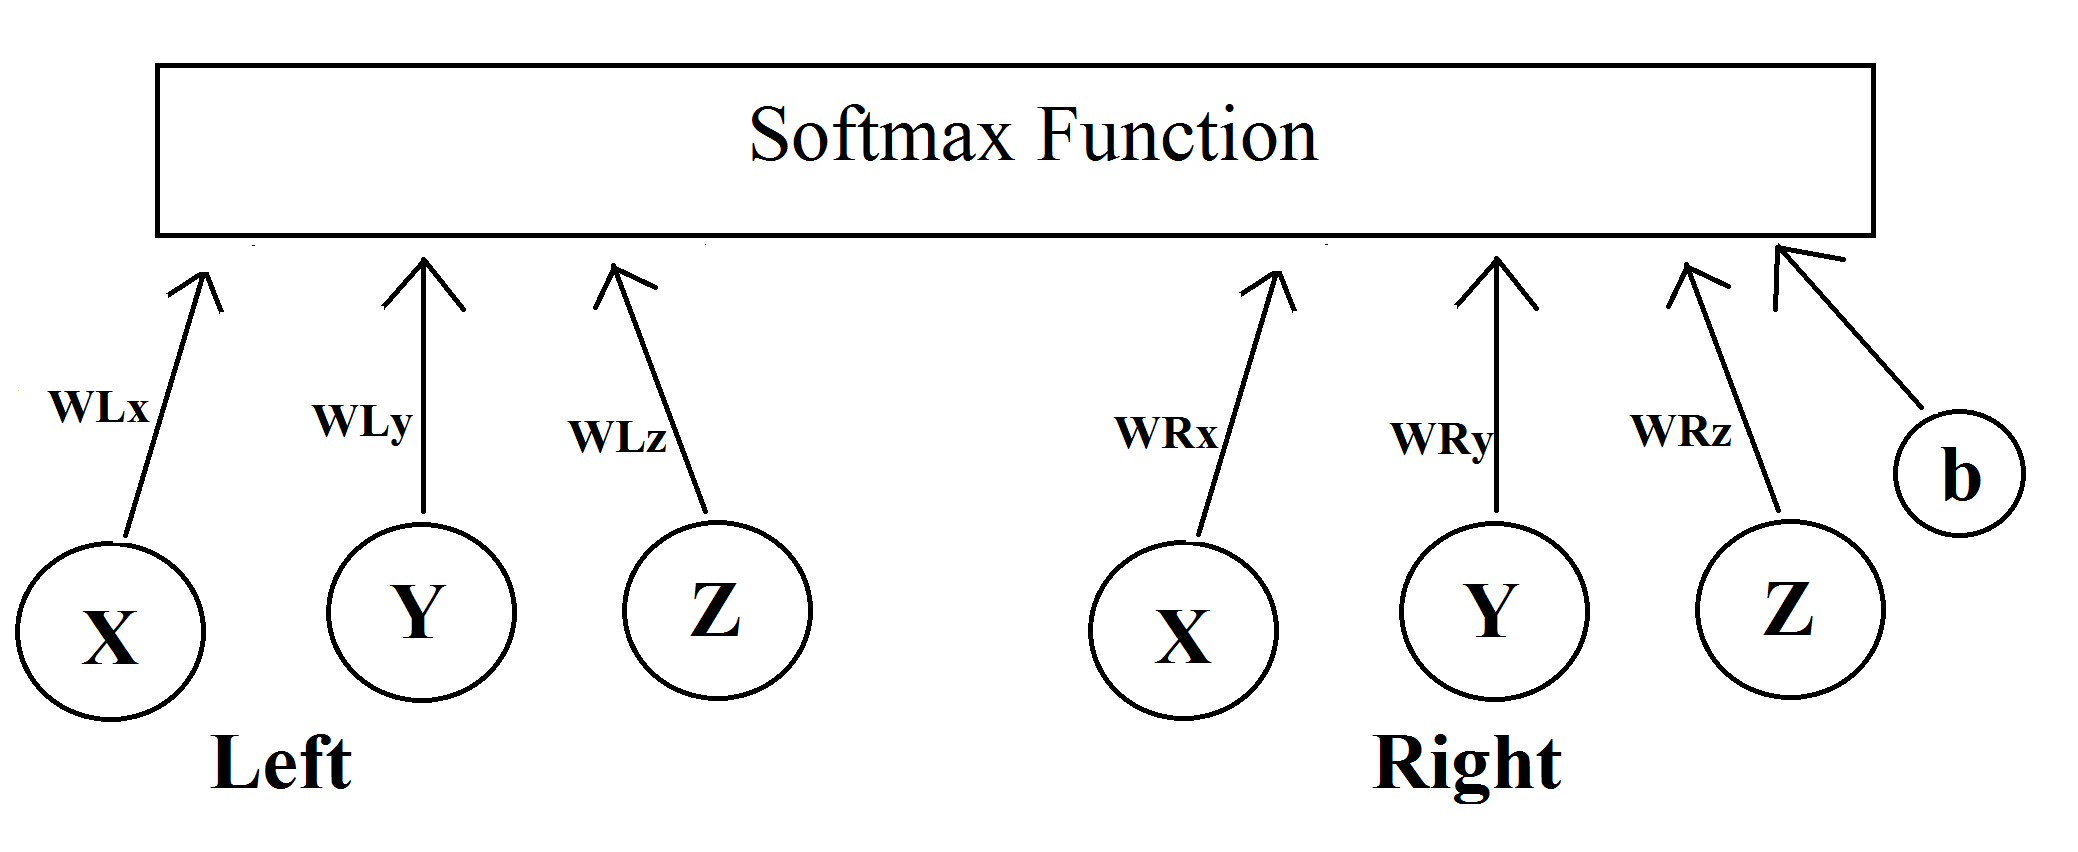
\includegraphics[width=0.5\textwidth]{../images/original}
	\caption{The Original Model}
	\label{original-model}
\end{figure}
\begin{figure}
	\centering
	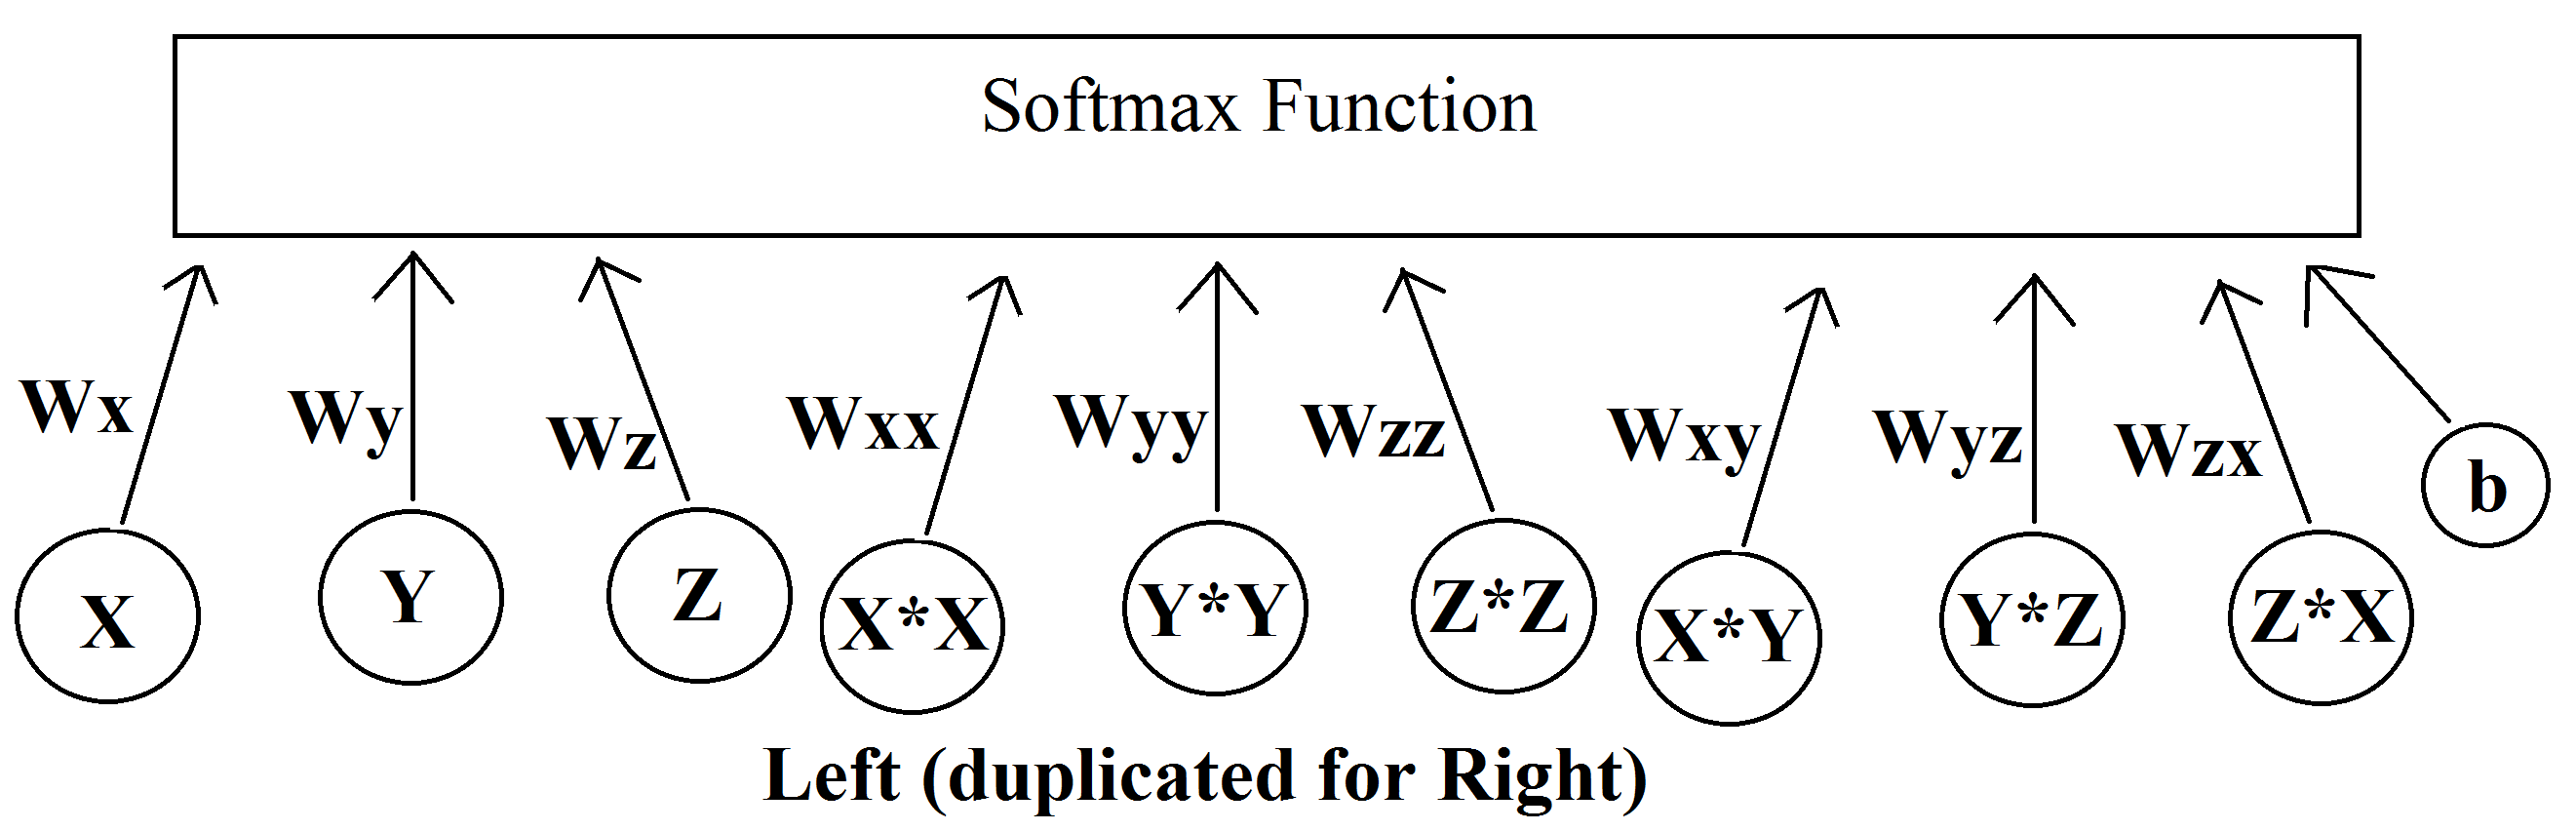
\includegraphics[width=0.5\textwidth]{../images/complex}
		\caption{The Complex Model}
	\label{complex-model}
\end{figure}
\begin{figure}
	\centering
	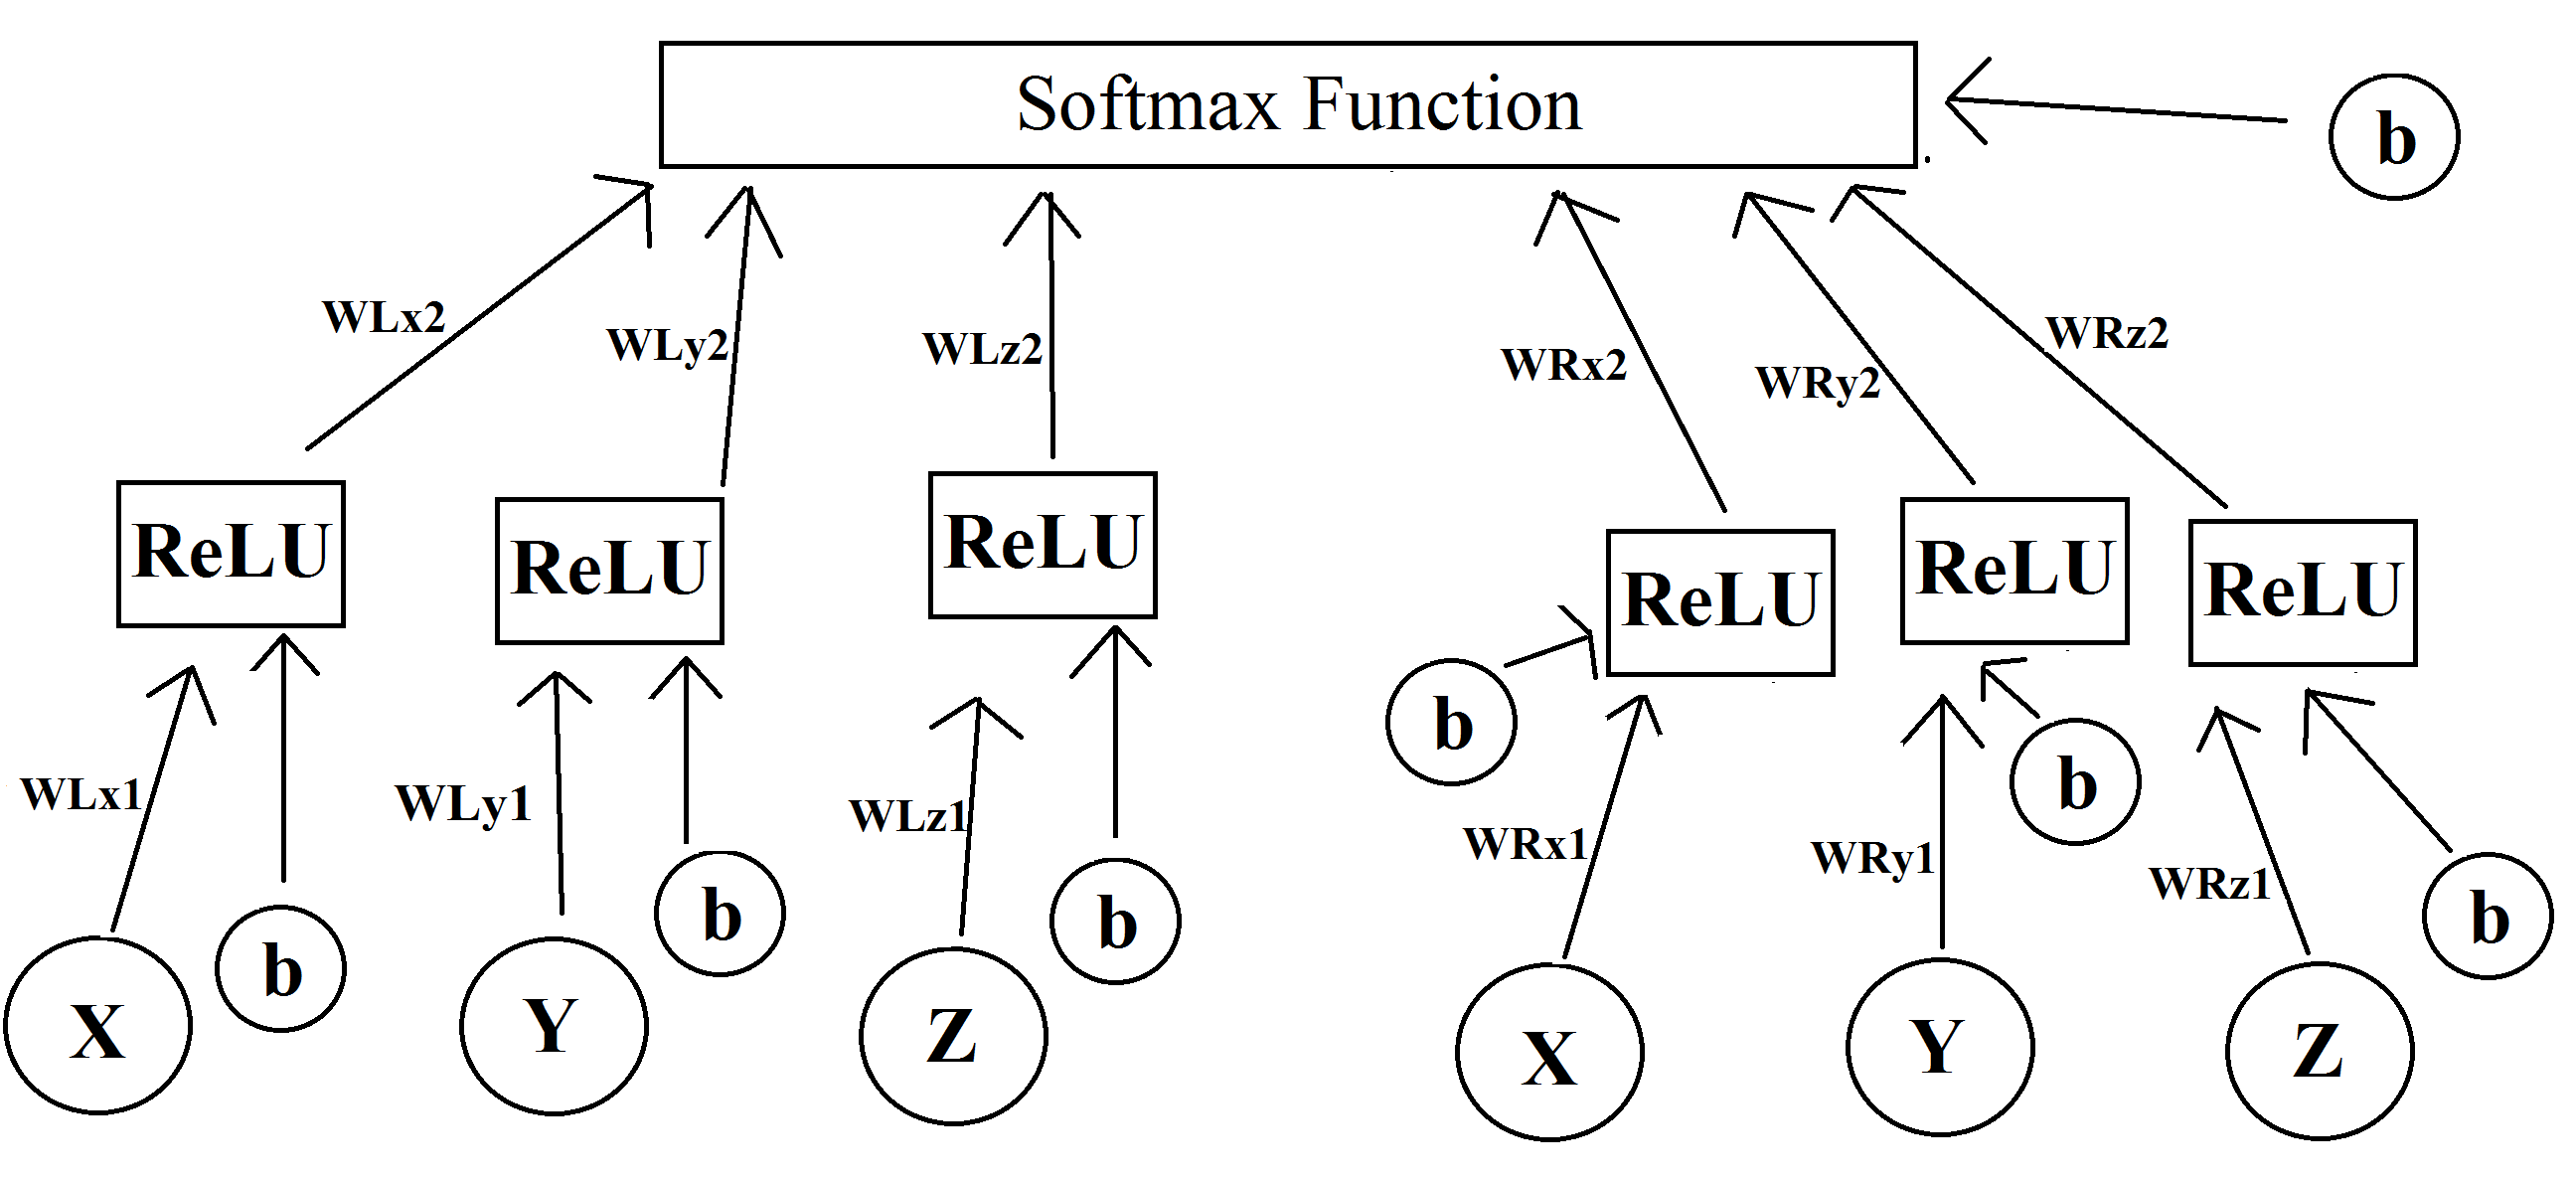
\includegraphics[width=0.5\textwidth]{../images/layered}
	\caption{The Layered Model}
	\label{layered-model}
\end{figure}
\begin{figure}
	\centering
	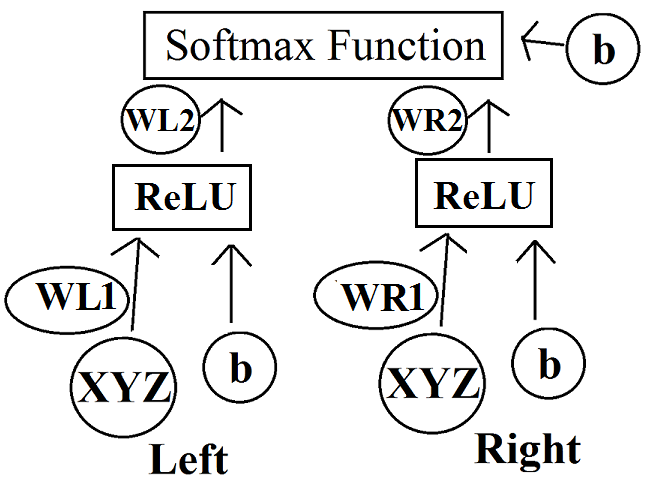
\includegraphics[width=0.5\textwidth]{../images/xyz1}
	\caption{The XYZ Model}
	\label{xyz-model}
\end{figure}
\begin{figure}
	\centering
	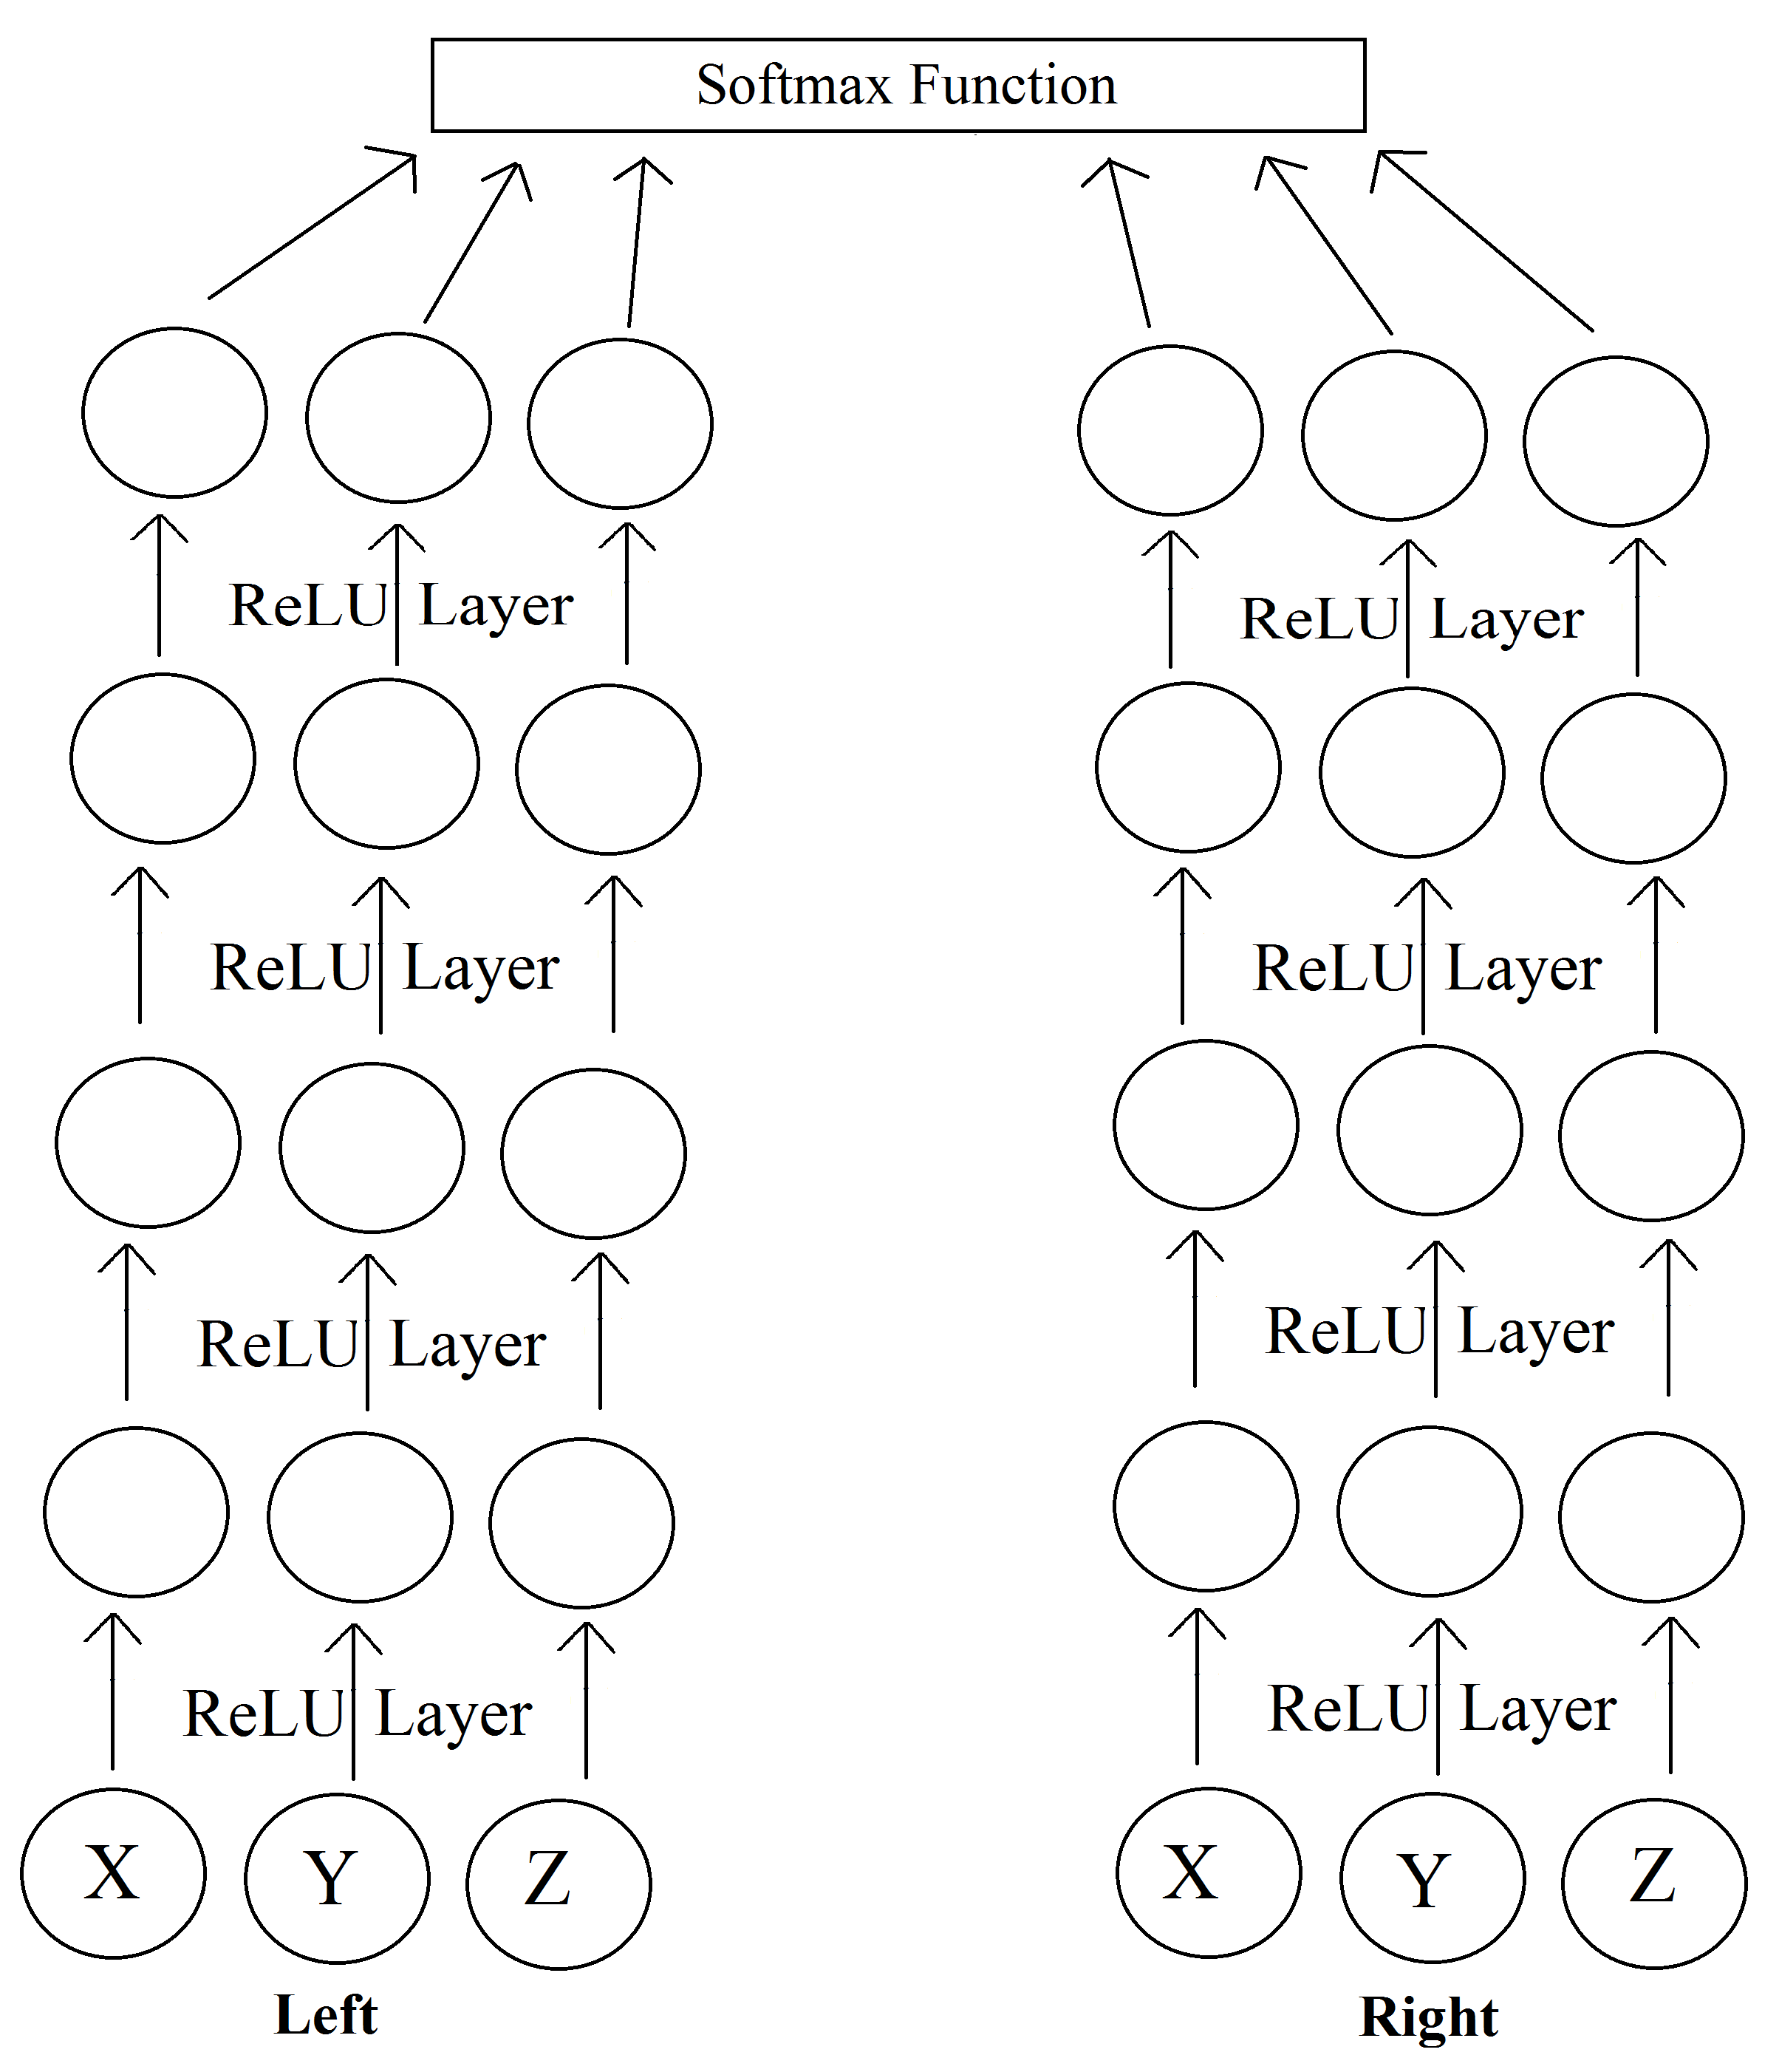
\includegraphics[width=0.5\textwidth]{../images/layered5}
	\caption{The 5-Layer Layered Model}
	\label{layered5-model}
\end{figure}
I then added a Convolutional Model, and I also added more layers to the Complex model and the Layered model in an attempt to improve accuracy. A simplified representation (removing some labels and not showing the bias vectors) of the additional layers in the Layered model is shown in Figure~\ref{layered5-model}.

\begin{figure}
	\centering
	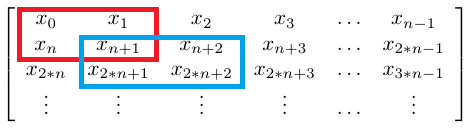
\includegraphics[width=0.5\textwidth]{../images/conv-issue}
	\caption{Sample Illustration of the Patch in a Convolutional Neural Network}
	\label{conv-issue}
\end{figure}
The convolutional model was an attempt to think of the X,Y,Z acceleration data as something akin to an RGB picture. I used 3 channels (for the X, Y, and Z data) as well as dropout for regularization. Nevertheless, this model had the worst performance overall, with the accuracy of the both-hands model coming in at under 50\%, shown later in Figure~\ref{acuracy-deep}. I have reasoned out that thinking about the data in this way just did not work within the framework of a convolutional neural network because while pictures can take advantage of the vertical and horizontal relationship between the data points, the time series data could not utilize and could be detrimentally affected by the vertical (non) relationship between the samples, illustrated in Figure~\ref{conv-issue}.

On the other hand, the XYZ model had too much success. It usually reached over 99.5\% accuracy, which told me that something was off. After discussion with my advisors, I have hypothesized that the layout of the data, shown in Figure~\ref{xyz-data}, combined with the super-sampling I did to increase the percentage of HH samples, worked out to make any given hand-hygiene sample have too many repeated values. I have assumed that this repetition led to easy identification of the hand-hygiene samples for the system, causing the almost impossibly high accuracy. Indeed, when I reduced the supersampling value in testing, results were markedly lower.

\begin{figure}
	\centering
	$$
	\left[
	\begin{array}{cccccccccccccc}
	x_{1} & y_{1} & z_{1} & x_{2} & ... & x_{n+1} & y_{n+1} & z_{n+1} & x_{n+2} & ... & x_{2*n+1} & y_{2*n+1} & ... & z_{3*n} \\
	x_{n+1} & y_{n+1} & z_{n+1} & x_{n+2} & ... & x_{2*n+1} & y_{2*n+1} & z_{2*n+1} & x_{2*n+2} & ... & x_{3*n+1} & y_{3*n+1} & ... & z_{4*n} \\
	\vdots & & (previous) & & \vdots & & (now) & &  & \vdots & & (next) & \ddots\\
	\end{array}
	\right]
	$$
	\caption{The XYZ Data Layout}
	\label{xyz-data}
\end{figure}


\section{Other Techniques}

With the models which had multiple layers, I also implemented L2 regularization. This technique attempts to prevent overfitting by reducing the total value of the weight matrices. Thus the model cannot become overtrained on the training data and score lower on the testing data.

Early stopping was another technique used to achieve higher accuracy. For this method, intermediate values of testing cross-entropy can be kept while the model is trained. In the event that testing cross-entropy suddenly spikes up (showing that a valley had been reached and then was essentially jumped over in the backpropagation process), the training can stop early and the previous, low testing error can be recorded.

\chapter{Results}

This part covers the results of the experiments I ran, described in the previous part of this thesis.

\section{Recall}

For all the tests I ran, I recorded statistics gathered from the confusion matrix. One of the main values one can gather from a confusion matrix is recall, which is $\frac{truepositives}{truepositives + falsenegatives}$. For this project, true positives are correctly-identified HH samples. False negatives are HH samples which were incorrectly identified as NHH samples. These values are all the averages from the models which took in the data of both the left and right hands as inputs. These values are from the testing portions of 10-fold cross-validated data. As shown in Figure~\ref{recall}, the 5 Layered model performed the best over all of the sample lengths, maxing out at 81.45\% recall with a sample length of 125 (= 1.25 seconds). The highest single value for recall was in the 5 Layered Complex model with 83.15\% recall at the sample length of 250. 

\begin{figure}
	\centering
	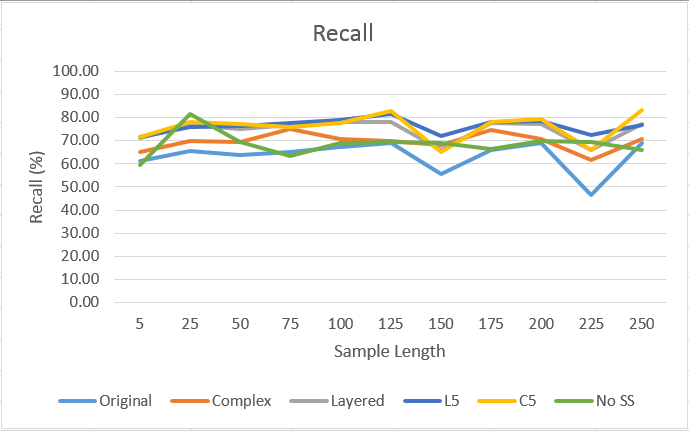
\includegraphics[width=0.5\textwidth]{../images/recall2}
	\caption{Recall Results}
	\label{recall}
\end{figure}

\section{Accuracy}

The accuracy results simple look at the percentage of total samples classified accurately. Overall these results were higher than the recall results, which is understandable since the accuracy values include the NHH samples. Again, the Layered 5 model achieved the highest results, shown in Figure~\ref{accuracy}. The maximum value on the 5 Layered model was an accuracy of 84.956\% with sample length 50. Not surprisingly the 5 Layered Complex model also performed quite well: the best accuracy result for that model was 84.75\%.

In Figure~\ref{acuracy-deep}, the less-than-stellar results for the Convolutional Model can be seen. As explained in Section~\ref{models}, setting up the data as a ``3-channel'' matrix did not perform well due to the lack of a ``vertical'' relationship of the time-based data.
\begin{figure}
	\centering
	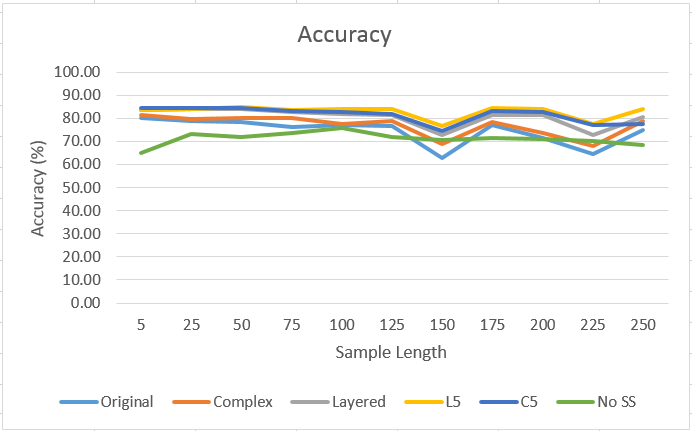
\includegraphics[width=0.5\textwidth]{../images/accuracy2}
	\caption{Accuracy Results}
	\label{accuracy}
\end{figure}
\begin{figure}
	\centering
	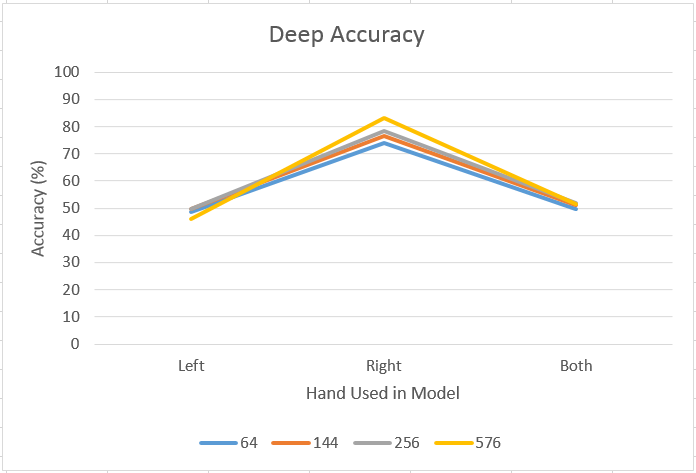
\includegraphics[width=0.5\textwidth]{../images/deepresults}
	\caption{Deep Model Accuracy}
	\label{acuracy-deep}
\end{figure}

\section{Other Notes}

The reader may have noticed the dips in the charts for the sample lengths of 150 and 225. I found this drop quite fascinating and I can only hypothesize that these sample lengths just did not ``line up'' well with the periodic motion of hand washing, which led to the poor results for these values. It is also interesting that the sample lengths immediately before and after these values rebounded and had results comparable to the other, shorter sample lengths.

Another note is the the ``No SS'' line in each of the above graphs represents the results for data which was not supersampled. To acheive a relatively even class balance, I had to remove almost all of the NHH data. This data loss can also account for the relatively poor / uneven performance between the different sample lengths: there simply was not enough data to fit the problem well. Indeed, some of the individual folds of the 10-fold cross validation process attained well below 50\% accuracy.

One interesting view is to look at the results by handedness, shown in Figure~\ref{handedness-original} for the Original Model and Figure~\ref{handedness-complex} for the Complex Model. In general the model that only used the left hand's data performed worse than those using only the right hand or both hands' data. It would certainly make sense that using both hands would be better than only one hand, but it is also a bit surprising that looking at only the right hand was so much better than the left hand, and was virtually on par with using both hands. I can certainly see that the right hand being the dominant hand for most people may help out the system to recognize activities in some way, and I would even invite the reader to attempt the motion for himself or herself to see which hand moves more.

\begin{figure}
	\centering
	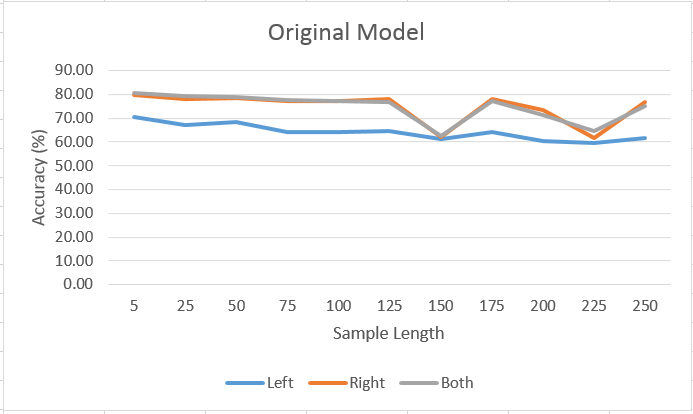
\includegraphics[width=0.5\textwidth]{../images/handed2o}
	\caption{Accuracy By Hand for the Original Model}
	\label{handedness-original}
\end{figure}
\begin{figure}
	\centering
	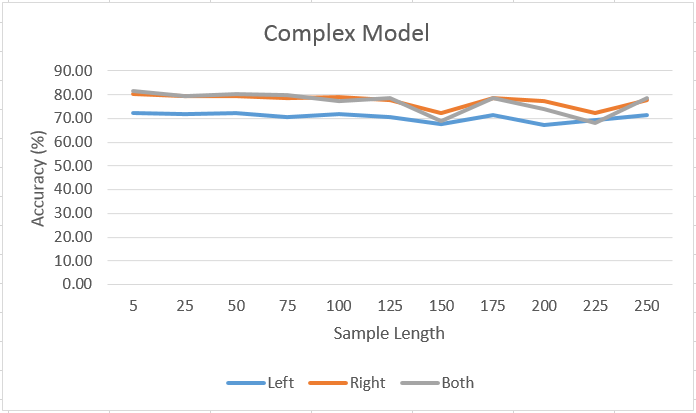
\includegraphics[width=0.5\textwidth]{../images/handed2c}
	\caption{Accuracy By Hand for the Original Model}
	\label{handedness-complex}
\end{figure}

\chapter{Discussion}

Now that the reader is familiar with my experiment and the results of it, I will enter into some discussion about the impact of what I have done as well as future work that could be done in this vein.

\section{Impact}

The main motivation for this work was to find a better way to ensure that healthcare workers are adequately washing their hands to prevent the spread of diseases in hospitals. While my best result of 85\% is by no means a perfect 100\%, I feel that this system would be an important first step to increasing the amount of times a healthcare worker would wash his or her hands.

One important factor is using the wrist-sensor system compared to any other would be the cost. These sensors would not be too expensive to produce, and would definitely be cheaper (and perhaps more accurate) than installing special sensors near every sink or hand sanitizer dispenser and then constructing a system to measure the amount of time a doctor or nurse is within a certain distance of a hand-washing location.

\section{Future Work}

If one were interested in further developing the physical system, it could be interesting to investigate using different sensors, such as velocity, relative location, and/or angular acceleration, and determining if a particular combination is more accurate at measuring hand hygiene.

Of course, one could also try to develop a more complicated neural network model or implement future deep learning techniques in order to improve the recall and accuracy of the system.

Another important area to look into would be utilizing a video input of hand movements, perhaps with a depth camera or just an RGB camera. The video input could also be combined with acceleration data for increased effectiveness.

Something else to look into would identifying proper hand hygiene technique, compared to simply detecting ``handwashing or not'' for a particular sample. Measuring the effectiveness of the hand hygiene may need many more sensors, as discussed above. It could also be difficult to express proper technique in a way that would generalize for many subjects.




%$$
%\left[
%\begin{array}{cccc}
%x_{1} & x_{2} & ... & x_{n} \\
%x_{n+1} & x_{n+2} & ... & x_{2*n} \\
% \vdots & & \ddots & \\
%\end{array}
%\right]
%$$




\bibliographystyle{plain}
\bibliography{./bibfile}
\end{document}          
